\documentclass[11pt, a4paper,twocolumn]{jarticle}
\usepackage[dvipdfmx]{graphicx}
\begin{document}
%=============================================================
\section{光学系の構築 (1日目)}
\subsection{実験目的}
今回の実験目的は光学系のアライメントを正確に行うことと,構築した光学系を用いてビーズのトラッピングを行うことである.

\subsection{実験手順}
まずダイヤルを回して出力電流を変えることでレーザー光の強さを調節した.
次にミラーを2枚用いてレーザー光を光学顕微鏡へ導入し,顕微鏡後側と対物レンズリボルバーに貼り付けられた的の真ん中にレーザー光が通過するようにミラーの位置と角度を調節した.
次にステージにスライドガラスを置いた後,リボルバーに水浸対物レンズを装着し,その上に蒸留水を2滴垂らした.またこのとき補正環は0.17に設定した.
さらに顕微鏡に入射した光がダイクロイックミラーによって試料ステージに反射されるように設定した.
その後CCDカメラによってレーザーがスライドガラス上に集光されることを確認した.
同心円状に集光できているかを確認し,モニターで映し出される集光スポットの中心にシールで目印を付けた.
次にミラーと顕微鏡の間にビームエキスパンダーを挿入し,同心円状に集光するまでビームエキスパンダーの位置の調整を行った.
完成した光学系は図\ref{fig:1}のようになった.

\begin{figure}[htbp]
 \begin{center}
  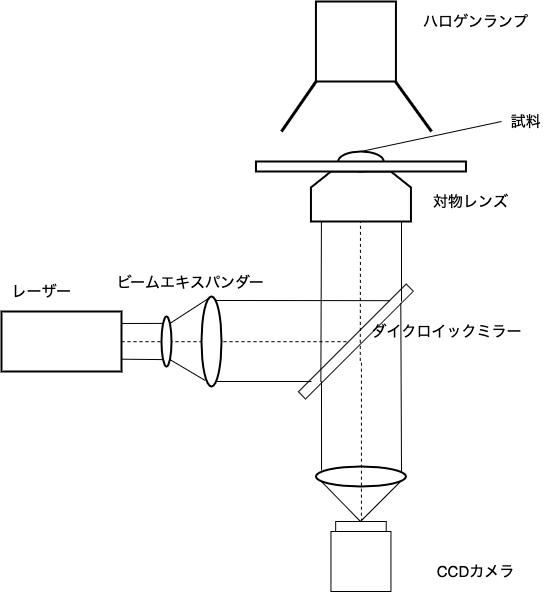
\includegraphics[width=0.8\linewidth]{fig1.png}
 \end{center}
 \caption{実験の光学系}
 \label{fig:1}
\end{figure}

\begin{figure}[htbp]
 \begin{center}
  \includegraphics[width=0.8\linewidth]{fig1-1.png}
 \end{center}
 \caption{同心円状パターン}
 \label{fig:1-1}
\end{figure}

\subsection{結果}
光学系の調整を行った図\ref{fig:1-1}のような同心円状の集光パターンが得られた.
また対物レンズの位置をスライドガラスを置いた試料ステージに近づけていくと2箇所で集光した.



\subsection{考察}
まずビームエキスパンダーを設置した理由について考察する.
レザー光は凸レンズに入射する事で一点に集光するがある程度の広がりを持つ.この時のスポット径を$d_0$,レンズの焦点距離f,レーザー波長$\lambda$,開口の直径をD,媒質の屈折率をnとすると以下の式で表せる.
\begin{equation}
    d = \frac{1.22f\lambda}{nD}
\end{equation}
よってビームエキスパンダーによってDの値を大きくする事でより集光スポットを小さくする目的があると考えられる.

さらに水侵対物レンズを用いる理由は対物レンズを抜けた光が進む媒質を水(n=1.33)にすることで集光スポット径をさらに小さくするためだと考えられる.

顕微鏡に入射した光をダイクロイックミラーで反射させたのは,ダイクロイックミラーが523nm以下の波長の光を透過して,それ以上の波長の光を反射させる性質を利用して,スライドガラスに反射したレザー光によって試料が観測できなくなる事を防ぐ目的であると考えられる.

また,光学顕微鏡へレーザー光を導入するときにミラーを2枚使った理由は任意の座標に任意の方向から光を入射させるためにはミラーが2枚必要であるからだと考えられる.

集光した際に図\ref{fig:1-1}のような同心円状パターンが得られた理由は対物レンズで集光した際にレンズの外側を通過する光と内側を通過する光で光路差が異なるために干渉をおこしレンズ中心からの距離に応じて明線,暗線が生じたためだと考えられる.

%=============================================================
\newpage
\end{document}
